\begin{frame}{Research Training}
\framesubtitle{Linear Sensor Network}
\begin{figure}[H]
    \centering
    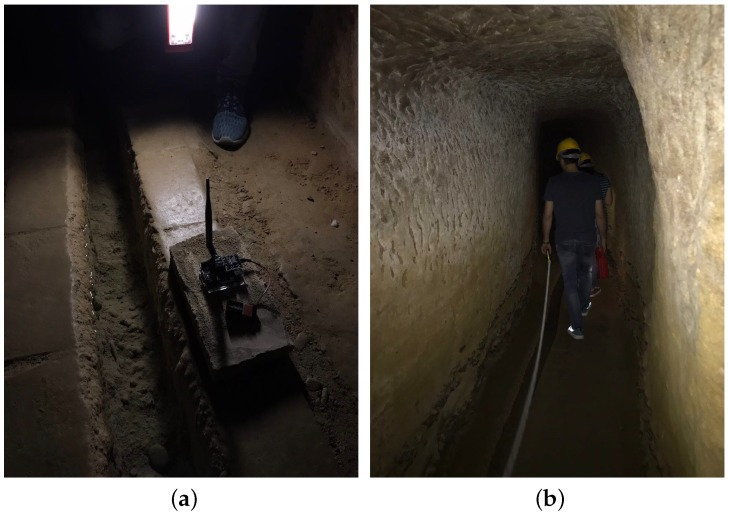
\includegraphics[width=0.7\textwidth]{presentation.tex/fig/lsnlora.jpg}
    \caption{Underground tunnel installation\footnotemark}
\end{figure}
\footcitetext{Abrardo_2019}
\end{frame}

\begin{frame}{Research Training}
\framesubtitle{Linear Sensor Network}
\begin{columns}
\begin{column}{0.5\textwidth}
\begin{figure}[H]
    \centering
    \scalebox{0.6}{%
    \begin{tikzpicture}
    \path[] (-5,0) edge (3,0);
    \node[] at (-4.5, 0.7) {$N_3$};
    \node[] at (-2.5, 0.7) {$N_2$};
    \node[] at (0, 0.7) {$N_1$};
    \node[motes] (a4) at (-4.5, 0) {};
    \node[motes] (a5) at (-2.5, 0) {};
    \node[motes] (a6) at (0, 0) {};
    \node[gateways] (a7) at (2.5, 0) {};
    \path (a4) edge [thick,bend left,dotted,->] node {     } (a5);
    \path (a5) edge [thick,bend left,dotted,->] node {     } (a6);
    \path (a6) edge [thick,bend left,dotted,->] node {     } (a7);

    % \draw[dotted,draw={black}] (-4.5,0) circle (3cm);
    \draw[dotted,draw={black}] (-2.5,0) circle (3cm);
    \draw[dotted,draw={black}] (0,0) circle (3cm);
    \end{tikzpicture}
    }
\end{figure}
\end{column}
\begin{column}{0.5\textwidth}
\begin{figure}[H] % TODO More info on axis
\centering
  \scalebox{0.6}{
  \begin{tikzpicture}[
    ack/.style={draw, rectangle, fill=orange!40, inner sep=0pt, outer sep=0pt},
    tx/.style={draw, rectangle, fill=blue!30,inner sep=0pt, outer sep=0pt},
    beacon/.style={draw, rectangle, fill=green!30,inner sep=0pt, outer sep=0pt},
    rx/.style={draw, pattern=north west lines, pattern color=black!60, rectangle, inner sep=0pt, outer sep=0pt},
    arr/.style={help lines,black!70,<->},
    ]
    \draw[->,thick] (-0.1,0)--(6,0) node[right]{time};
    \draw[->,thick] (0,-0.1)--(0,5) node[above]{};

    \draw[dotted] (-0.1,0.5)--(6,0.5);
    \node[] at (-1.2, 1) {Gateway};
    \draw[] (-0.1,1)--(0.1,1);
    \draw[dotted] (-0.1,1.5)--(6,1.5);
    \node[] at (-1.2, 2) {Node 1};
    \draw[] (-0.1,2)--(0.1,2);
    \draw[dotted] (-0.1,2.5)--(6,2.5);
    \node[] at (-1.2, 3) {Node 2};
    \draw[] (-0.1,3)--(0.1,3);
    \draw[dotted] (-0.1,3.5)--(6,3.5);
    \node[] at (-1.2, 4) {Node 3};
    \draw[] (-0.1,4)--(0.1,4);
    \draw[dotted] (-0.1,4.5)--(6,4.5);

    % Gateway
    \node () [rx, fit={(1.1,0.7) (1.4,1.3)}] {};
    \node () [rx, fit={(3.1,0.7) (3.4,1.3)}] {};
    \node () [rx, fit={(5.1,0.7) (5.4,1.3)}] {};
    % 1
    \node () [rx, fit={(0.8,1.7) (1.1,2.3)}] {};
    \node () [beacon, fit={(1.1,1.7) (1.4,2.3)}] {};

    \node () [rx, fit={(2.8,1.7) (3.1,2.3)}] {};
    \node () [tx, fit={(3.1,1.7) (3.4,2.3)}] {};

    \node () [rx, fit={(4.8,1.7) (5.1,2.3)}] {};
    \node () [tx, fit={(5.1,1.7) (5.4,2.3)}] {};
    % 2
    \node () [rx, fit={(0.5,2.7) (0.8,3.3)}] {};
    \node () [beacon, fit={(0.8,2.7) (1.1,3.3)}] {};

    \node () [rx, fit={(2.5,2.7) (2.8,3.3)}] {};
    \node () [tx, fit={(2.8,2.7) (3.1,3.3)}] {};

    \node () [rx, fit={(4.5,2.7) (4.8,3.3)}] {};
    \node () [tx, fit={(4.8,2.7) (5.1,3.3)}] {};
    % 3
    \node () [beacon, fit={(0.5,3.7) (0.8,4.3)}] {};
    \node () [tx, fit={(2.5,3.7) (2.8,4.3)}] {};
    \node () [tx, fit={(4.5,3.7) (4.8,4.3)}] {};

    \draw[arr,<->] (0.8, 4) -- node[fill=white] {\tiny $interval$} (2.5, 4);
  \end{tikzpicture}
  }
  % \caption{Collision between nodes}
  \scalebox{0.6}{
  \begin{tabular}{r@{ }l r@{ }l}
  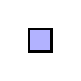
\begin{tikzpicture}\draw[fill=blue!30,line width=1pt] +(-4pt,-4pt) rectangle +(4pt,4pt);\end{tikzpicture} & Transmission 
    & 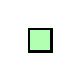
\begin{tikzpicture}\draw[fill=green!30,line width=1pt] +(-4pt,-4pt) rectangle +(4pt,4pt);\end{tikzpicture} & Synchronization \\
  \begin{tikzpicture}\draw[pattern=north west lines, pattern color=black!90,line width=1pt] +(-4pt,-4pt) rectangle +(4pt,4pt);\end{tikzpicture} & Reception
  \end{tabular}
  }
\end{figure}
\end{column}
\end{columns}
\end{frame}

\begin{frame}{Research Training}
\framesubtitle{LoRaBlink}
\begin{columns}
\begin{column}{0.5\textwidth}
\begin{figure}[H]
    \centering
    \scalebox{0.8}{
    \begin{tikzpicture}[auto, thick]
      \foreach \place/\name in {{(0,0)/a}}
        \node[gateways] (\name) at \place {};

      \node[] at (-2.0, 1.2) {$N_2$};
      \node[motes] (a4) at (-1.6, 1.2) {};
      \node[] at (-2.2, 3.3) {$N_3$};
      \node[motes] (a5) at (-1.8, 3.3) {};
      \node[] at (-1.2, 0.7) {$N_1$};
      \node[motes] at (-0.8, 0.8) (a6) {};
      \node[motes] (a7) at (1, 1.5) {};
      \node[motes] (a8) at (1.2, 3) {};
      \node[motes] (a9) at (0.2, 2) {};

      \path[dotted,->] (a5) edge (a4);
      \path[dotted,->] (a4) edge (a6);
      \path[dotted,->] (a6) edge (a);

      \path[dotted,->] (a9) edge (a);
      \path[dotted,->] (a8) edge (a7);
      \path[dotted,->] (a7) edge (a);
    \end{tikzpicture}
    }
    \caption{}
    \scalebox{0.6}{%
    \begin{tabular}{r@{: }l r@{: }l}
    
\begin{tikzpicture}\draw[left color=orange,line width=1pt] circle(1ex);\end{tikzpicture} & Gateway & 
\begin{tikzpicture}\draw[left color=gray,line width=1pt] circle(1ex);\end{tikzpicture} & Mote
    \end{tabular}
    }
\end{figure}
\end{column}
\begin{column}{0.5\textwidth}
\begin{figure}[H] % TODO More info on axis
\centering
  \scalebox{0.6}{
  \begin{tikzpicture}[
    ack/.style={draw, rectangle, fill=orange!40, inner sep=0pt, outer sep=0pt},
    tx/.style={draw, rectangle, fill=blue!30,inner sep=0pt, outer sep=0pt},
    relay/.style={draw, rectangle, fill=green!30,inner sep=0pt, outer sep=0pt},
    rx/.style={draw, pattern=north west lines, pattern color=black!60, rectangle, inner sep=0pt, outer sep=0pt},
    arr/.style={help lines,black!70,<->},
    ]
    \draw[->,thick] (-0.1,0)--(6,0) node[right]{time};
    \draw[->,thick] (0,-0.1)--(0,5) node[above]{};

    \draw[dotted] (-0.1,0.5)--(6,0.5);
    \node[] at (-1.2, 1) {Gateway};
    \draw[] (-0.1,1)--(0.1,1);
    \draw[dotted] (-0.1,1.5)--(6,1.5);
    \node[] at (-1.2, 2) {Node 1};
    \draw[] (-0.1,2)--(0.1,2);
    \draw[dotted] (-0.1,2.5)--(6,2.5);
    \node[] at (-1.2, 3) {Node 2};
    \draw[] (-0.1,3)--(0.1,3);
    \draw[dotted] (-0.1,3.5)--(6,3.5);
    \node[] at (-1.2, 4) {Node 3};
    \draw[] (-0.1,4)--(0.1,4);
    \draw[dotted] (-0.1,4.5)--(6,4.5);

    % Gateway
    \node () [rx, fit={(1.1,0.7) (1.4,1.3)}] {};
    \node () [rx, fit={(3.1,0.7) (3.4,1.3)}] {};
    \node () [rx, fit={(5.1,0.7) (5.4,1.3)}] {};
    % 1
    \node () [rx, fit={(1.1,1.7) (1.4,2.3)}] {};
    \node () [rx, fit={(3.1,1.7) (3.4,2.3)}] {};
    \node () [relay, fit={(5.1,1.7) (5.4,2.3)}] {};
    % 2
    \node () [rx, fit={(1.1,2.7) (1.4,3.3)}] {};
    \node () [relay, fit={(3.1,2.7) (3.4,3.3)}] {};
    \node () [rx, fit={(5.1,2.7) (5.4,3.3)}] {};
    % 3
    \node () [tx, fit={(1.1,3.7) (1.4,4.3)}] {};
    \node () [rx, fit={(3.1,3.7) (3.4,4.3)}] {};
    \node () [rx, fit={(5.1,3.7) (5.4,4.3)}] {};
    % \node () [beacon, fit={(0.5,3.7) (0.8,4.3)}] {};
    % \node () [tx, fit={(2.5,3.7) (2.8,4.3)}] {};
    % \node () [tx, fit={(4.5,3.7) (4.8,4.3)}] {};
  \end{tikzpicture}
  }
  % \caption{Collision between nodes}
  \scalebox{0.6}{
  \begin{tabular}{r@{ }l r@{ }l}
  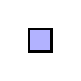
\begin{tikzpicture}\draw[fill=blue!30,line width=1pt] +(-4pt,-4pt) rectangle +(4pt,4pt);\end{tikzpicture} & Transmission 
    & 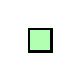
\begin{tikzpicture}\draw[fill=green!30,line width=1pt] +(-4pt,-4pt) rectangle +(4pt,4pt);\end{tikzpicture} & Relay \\
  \begin{tikzpicture}\draw[pattern=north west lines, pattern color=black!90,line width=1pt] +(-4pt,-4pt) rectangle +(4pt,4pt);\end{tikzpicture} & Reception
  \end{tabular}
  }
\end{figure}
\end{column}
\end{columns}
\footcitetext{lorablink}
\end{frame}

\begin{frame}{Research Training}
\framesubtitle{LoRaWAN Extension}
\begin{columns}
\begin{column}{0.5\textwidth}
\begin{figure}[H]
\centering
\scalebox{0.7}{
\begin{tikzpicture}[auto, thick]
    \foreach \place/\name in {{(0,0)/a}}
        \node[gateways] (\name) at \place {};
    % Place normal peers
    \foreach \pos/\i in {below left of/1, below of/2, left of/3, above left of/4, below right of/5,above of/6, right of/7, above right of/8}
        \node[motes, \pos =a ] (a\i) {};
    \foreach \speer/\peer in {a/a1,a/a2,a/a3,a/a4,a/a5,a/a6,a/a7,a/a8}
        \path[dotted] (\speer) edge (\peer);
    \node[motes, left of=a3 ] (relay) {};
    \path[dotted] (relay) edge (a3);
\end{tikzpicture}
}
\caption{}
\scalebox{0.5}{%
\begin{tabular}{r@{ }l r@{ }l}

\begin{tikzpicture}\draw[left color=orange,line width=1pt] circle(1ex);\end{tikzpicture} & Gateway & 
\begin{tikzpicture}\draw[left color=gray,line width=1pt] circle(1ex);\end{tikzpicture} & Mote
\end{tabular}
}
\end{figure}
\end{column}
\begin{column}{0.5\textwidth}
\begin{figure}[H] % TODO More info on axis
\centering
  \scalebox{0.6}{
  \begin{tikzpicture}[
    ack/.style={draw, rectangle, fill=orange!40, inner sep=0pt, outer sep=0pt},
    tx/.style={draw, rectangle, fill=blue!30,inner sep=0pt, outer sep=0pt},
    relay/.style={draw, rectangle, fill=green!30,inner sep=0pt, outer sep=0pt},
    rx/.style={draw, pattern=north west lines, pattern color=black!60, rectangle, inner sep=0pt, outer sep=0pt},
    arr/.style={help lines,black!70,<->},
    ]
    \draw[->,thick] (-0.1,0)--(6,0) node[right]{time};
    \draw[->,thick] (0,-0.1)--(0,4) node[above]{};

    \draw[dotted] (-0.1,0.5)--(6,0.5);
    \node[] at (-1.2, 1) {Gateway};
    \draw[] (-0.1,1)--(0.1,1);
    \draw[dotted] (-0.1,1.5)--(6,1.5);
    \node[] at (-1.2, 2) {Relay};
    \draw[] (-0.1,2)--(0.1,2);
    \draw[dotted] (-0.1,2.5)--(6,2.5);
    \node[] at (-1.2, 3) {Node};
    \draw[] (-0.1,3)--(0.1,3);
    \draw[dotted] (-0.1,3.5)--(6,3.5);

    % Gateway
    \node () [rx, fit={(0.1,0.7) (5.9,1.3)}] {};
    % Relay
    \node () [rx, fit={(1.1,1.7) (1.4,2.3)}] {};
    \node () [rx, fit={(3.1,1.7) (3.4,2.3)}] {};
    \node () [rx, fit={(5.1,1.7) (5.4,2.3)}] {};
    \node () [relay, fit={(5.4,1.7) (5.7,2.3)}] {};
    % Node
    \node () [tx, fit={(5.1,2.7) (5.4,3.3)}] {};
    % \node () [beacon, fit={(0.5,3.7) (0.8,4.3)}] {};
    % \node () [tx, fit={(2.5,3.7) (2.8,4.3)}] {};
    % \node () [tx, fit={(4.5,3.7) (4.8,4.3)}] {};
  \end{tikzpicture}
  }
  % \caption{Collision between nodes}
  \scalebox{0.6}{
  \begin{tabular}{r@{ }l r@{ }l}
  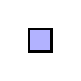
\begin{tikzpicture}\draw[fill=blue!30,line width=1pt] +(-4pt,-4pt) rectangle +(4pt,4pt);\end{tikzpicture} & Transmission 
    & 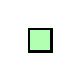
\begin{tikzpicture}\draw[fill=green!30,line width=1pt] +(-4pt,-4pt) rectangle +(4pt,4pt);\end{tikzpicture} & Relay \\
  \begin{tikzpicture}\draw[pattern=north west lines, pattern color=black!90,line width=1pt] +(-4pt,-4pt) rectangle +(4pt,4pt);\end{tikzpicture} & Reception
  \end{tabular}
  }
\end{figure}
\end{column}
\end{columns}
\footcitetext{DIAS2018424}
\end{frame}
